%%----------------------------------------------------------------------------------------
%	PACKAGES AND THEMES
%----------------------------------------------------------------------------------------
\PassOptionsToPackage{table}{xcolor}
\documentclass[aspectratio=169,xcolor=dvipsnames,svgnames,x11names,fleqn]{beamer}
% \documentclass[aspectratio=169,xcolor=dvipsnames,fleqn]{beamer}

\usetheme{RedVelvet}

\usefonttheme[onlymath]{serif}
\newcommand{\showanswers}{yes}
\usepackage{pifont} % For checkmarks and crosses

\usepackage{setspace}
\usepackage{xspace}
\usepackage{amsmath}
\usepackage{amssymb}
\usepackage{amsfonts}
\usepackage{color}
\usepackage{physics}
% \usepackage{mathbb}
\usepackage{rahul_math}
\usepackage{bigints}

\usepackage[utf8]{inputenc}
\usepackage[ruled,vlined]{algorithm2e}
\usepackage{amsmath}
\usepackage{amsfonts}

\usepackage{graphicx} % Allows including images
\usepackage{booktabs} % Allows the use of \toprule, \midrule and \bottomrule in tables
\usepackage{tikz,pgfplots}
\usepackage{mathtools}
\usepackage{subfigure}
\usetikzlibrary{arrows}
\usepackage{minted}
\definecolor{LightGray}{gray}{0.9}
\definecolor{cream}{rgb}{0.92, 0.9, 0.55}
\definecolor{lightblue}{rgb}{0.68, 0.85, 0.9}


\usepackage{xcolor-material}
\usetikzlibrary{fit}
\usetikzlibrary{matrix}
\tikzset{%
apple/.pic={
    \fill [MaterialBrown] (-1/8,0)  arc (180:120:1 and 3/2) coordinate [pos=3/5] (@)-- ++(1/6,-1/7)  arc (120:180:5/4 and 3/2) -- cycle;
    \fill [MaterialLightGreen500] (0,-9/10)  .. controls ++(180:1/8) and ++(  0:1/4) .. (-1/3,  -1) .. controls ++(180:1/3) and ++(270:1/2) .. (  -1,   0) .. controls ++( 90:1/3) and ++(180:1/3) .. (-1/2, 3/4) .. controls ++(  0:1/8) and ++(135:1/8) .. (   0, 4/7)
    }
    }

\newcommand{\leftdoublequote}{\textcolor{blue}{\scalebox{3}{``}}}

\newcommand{\rightdoublequote}{\textcolor{blue}{\scalebox{3}{''}}}


\usepackage{textcomp}
\usepackage{fontawesome}
\usepackage{tikz,pgfplots}
\usetikzlibrary{shapes.callouts}
\usetikzlibrary{arrows}
\usetikzlibrary{shapes.geometric, positioning}
\usetikzlibrary{matrix,positioning,decorations.pathreplacing,calc}
\usepackage{tikz-dependency}

\pgfplotsset{compat=1.8} % or newest version

\usetikzlibrary{positioning}


\usepackage{bm}
\usepackage{relsize}

\tcbuselibrary{skins, hooks}

\tikzset{basic/.style={draw,fill=MediumBlue!20,text width=1em,text badly centered}}
\tikzset{input/.style={basic,circle}}
\tikzset{weights/.style={basic,rectangle}}
\tikzset{functions/.style={basic,circle,fill=MediumBlue!10}}



\usepackage{listofitems} % for \readlist to create arrays
\tikzstyle{mynode}=[thick,draw=MediumBlue,fill=MediumBlue!20,circle,minimum size=22]


\usepackage{overpic}

%----------------------------------------------------------------------------------------
%	TITLE PAGE
%----------------------------------------------------------------------------------------

\usepackage{tikz-qtree,tikz-qtree-compat}
\usetikzlibrary{tikzmark}
\usetikzlibrary{calc}

\usetikzlibrary{fit}
\tikzset{%
apple/.pic={
    \fill [MaterialBrown] (-1/8,0)  arc (180:120:1 and 3/2) coordinate [pos=3/5] (@)-- ++(1/6,-1/7)  arc (120:180:5/4 and 3/2) -- cycle;
    \fill [MaterialLightGreen500] (0,-9/10)  .. controls ++(180:1/8) and ++(  0:1/4) .. (-1/3,  -1) .. controls ++(180:1/3) and ++(270:1/2) .. (  -1,   0) .. controls ++( 90:1/3) and ++(180:1/3) .. (-1/2, 3/4) .. controls ++(  0:1/8) and ++(135:1/8) .. (   0, 4/7)
}
}
\usepackage{tikz-qtree,tikz-qtree-compat}
\usetikzlibrary{tikzmark}
\usetikzlibrary{calc}

\usetikzlibrary{positioning}
\newcommand{\vect}[1]{\mathbf{#1}}
% Define styles
\tikzset{
    box/.style={
        rectangle,
        draw=black,
        fill=blue!20,
        text width=2.2cm,
        text centered,
        minimum height=0.8cm,
        font=\small
    },
    arrow/.style={
        ->,
        >=Stealth,
        line width=1.5pt,
        draw=black
    }
}


\usepackage{bm}
\usepackage{relsize}



\tikzset{basic/.style={draw,fill=MediumBlue!20,text width=1em,text badly centered}}
\tikzset{input/.style={basic,circle}}
\tikzset{weights/.style={basic,rectangle}}
\tikzset{functions/.style={basic,circle,fill=MediumBlue!10}}
\usetikzlibrary{arrows.meta, bending}
\usetikzlibrary{shapes.geometric, arrows.meta, positioning, fit, backgrounds}

\usepackage{listofitems} % for \readlist to create arrays
\tikzstyle{mynode}=[thick,draw=MediumBlue,fill=MediumBlue!20,circle,minimum size=22]


\newmdenv[
backgroundcolor=androidYellowLight,
linecolor=androidYellow,
linewidth=0.5pt,
roundcorner=10pt,
skipabove=\baselineskip,
skipbelow=\baselineskip
]{MintedFrame}

% Set minted options
\setminted{
fontsize=\footnotesize,
breaklines=true,
autogobble,
linenos,
frame=none
}


\title[CPE 487/587: Deep Learning]{CPE 486/586: Deep Learning for Engineering Applications} % The short title appears at the bottom of every slide, the full title is only on the title page
\subtitle{11 Graph Neural Network}

\author[Rahul Bhadani] {{\Large \textbf{Rahul Bhadani}}}

\institute[UAH] % Your institution as it will appear on the bottom of every slide, maybe shorthand to save space
{
    Electrical \& Computer Engineering,  The University of Alabama in Huntsville
}
\date

% \titlegraphic{
%    \includegraphics[width=0.4\linewidth]{figures/UAH_primary.png}
% }



\begin{document}

%-------------------------------------------------
\begin{frame}
    \titlepage
\end{frame}

%-------------------------------------------------
\begin{frame}{Outline}
    \backgroundtableofcontents
\end{frame}

%------------------------------------------------
\section{Motivation}
%------------------------------------------------


\begin{frame}{}
    \begin{center}
    \huge \bf \color{DarkBlue}
    Motivation        
\end{center}
\end{frame}

\begin{frame}{Graph/Network Dataset}

\begin{center}
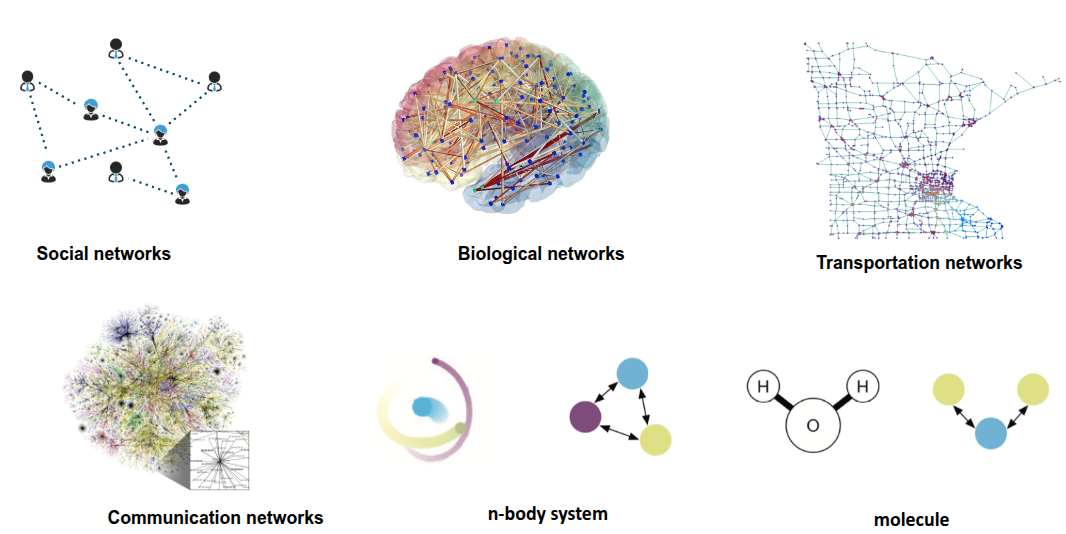
\includegraphics[width=0.78\linewidth]{figures/networks.png}
\end{center}


\end{frame}


\begin{frame}{Graph/Network Dataset}

\begin{center}
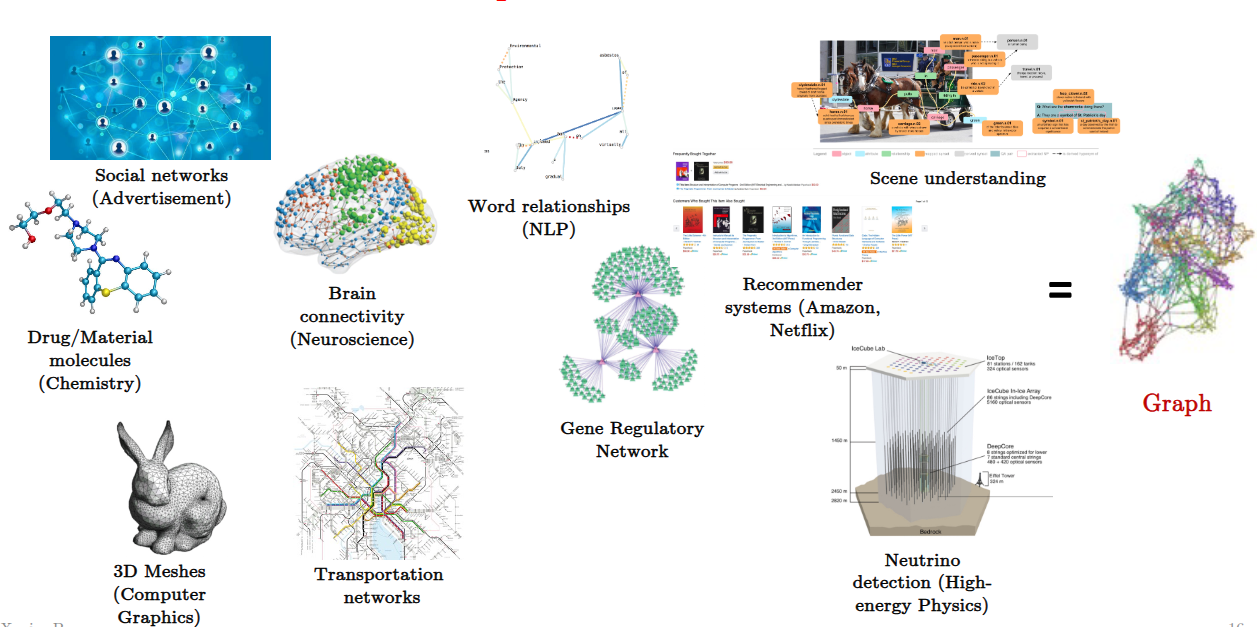
\includegraphics[width=0.78\linewidth]{figures/networks2.png}
\end{center}


\end{frame}


\begin{frame}{Graphs to Represent Dataset}

\begin{columns}

\column{0.5\linewidth}

\begin{itemize}
\item Graphs can be used to represent relationships in a structured data.
\item They provide a different perspective of dataset.
\item Impose relational inductive bias in data
\item Lead to knowledge discovery
\end{itemize}


\column{0.5\linewidth}
\begin{center}
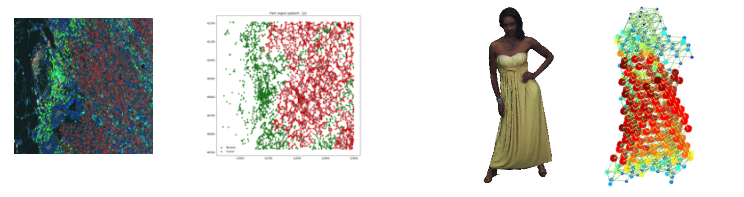
\includegraphics[width=0.9\linewidth]{figures/graph_models_1.png}


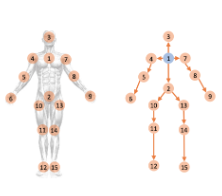
\includegraphics[width=0.4\linewidth]{figures/graph_models_2.png}

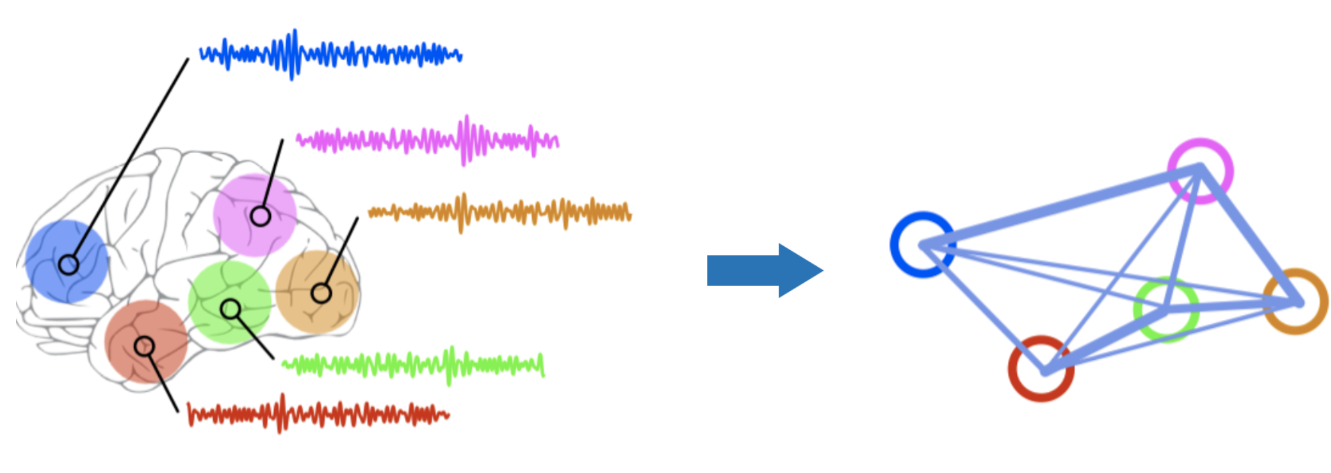
\includegraphics[width=0.6\linewidth]{figures/graph_models_3.png}

\end{center}

\end{columns}

\end{frame}




\begin{frame}{What is Graph?}

\footnotesize

\begin{center}
A graph $G$ is a data structure described by a set of edges and vertices (also known as nodes):

$$
G = (V, E) \text{~~~ or ~~~~} G = (V, E, A)
$$
\end{center}


\begin{itemize}
\item $V$ set of vertices.
\item $E$ set of edges.
\item They can be directed or undirected.
\end{itemize}

\begin{center}
A graph is often represented by an Adjacency matrix, $A$. If a graph has $N$ nodes, then $A$ has a dimension of $(N\times N)$. People sometimes provide another feature matrix to describe the nodes in the graph. If each node has F numbers of features, then the feature matrix $X$ has a dimension of $(N\times F)$.

\resizebox{0.2\linewidth}{!}{
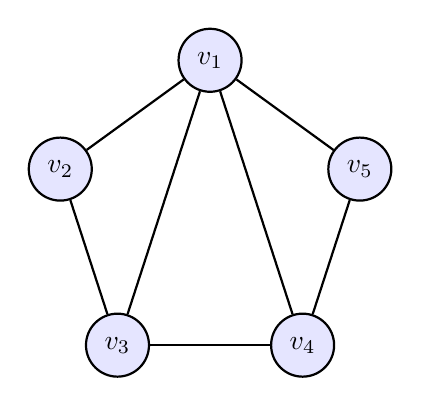
\begin{tikzpicture}[
    % Defining global styles for our vertices
    every node/.style={
        circle, 
        draw=black, 
        fill=blue!10, 
        thick, 
        minimum size=8mm
    },
    % Defining style for our edges
    edge style/.style={
        draw=black, 
        thick
    }
]

    % Place vertices in a circular layout
    \foreach \i in {1,...,5} {
        \node (\i) at ({72 * (\i - 1) + 90}:2cm) {$v_{\i}$};
    }

    % Draw edges manually to show specific connections
    \begin{scope}[edge style]
        \draw (1) -- (2);
        \draw (2) -- (3);
        \draw (3) -- (4);
        \draw (4) -- (5);
        \draw (5) -- (1);
        
        % Adding internal chords to make it a "Graph Theory" example
        \draw (1) -- (3);
        \draw (1) -- (4);
    \end{scope}

\end{tikzpicture}
}

\end{center}


\end{frame}

\begin{frame}{What is Graph?}

Graph features:

\begin{itemize}
\item Node features: $h_i$, $h_j$ (e.g. Atom Type)
\item Edge features: $e_{ij}$ (e.g. bond type, time to travel from one traffic intersection to another, etc.)
\item Overall graph features: $g$ (e.g. molecular energy)
\end{itemize}

\end{frame}

\begin{frame}{Graphs are non-Euclidean Data}

\begin{center}
Suitable for data that resides in irregular, non-grid-like structures where relationships are not confined to regular
Euclidean spaces.
\end{center}

\vspace{10pt}

\begin{itemize}
\item Manifolds: Curved surfaces, e.g., 3D shapes or mesh data.
\item Point Clouds: Sets of points in 3D space without a grid
structure (e.g., LiDAR data).
\end{itemize}

\vspace{10pt}

Real-World Data is Often Non-Euclidean.


\end{frame}



\begin{frame}{Challenges in handling Non-Euclidean Data}

\footnotesize

\begin{itemize}
\item fixed Grid Assumptions in MLPs, CNNs, RNNs
\begin{itemize}
\item Assume regular, structured data (e.g., grids or
sequences).
\item Cannot directly handle irregular neighborhoods or
variable node connectivity in graphs or other
non-Euclidean structures.
\end{itemize}
\item Irregular Neighborhoods:
\begin{itemize}
\item Varying numbers of neighbors per node.
\item No uniform notion of proximity or direction.
\item Standard convolution filters (which operate on fixed local
neighborhoods) fail to adapt to these variable structures.
\end{itemize}
\item Lack of Spatial Regularity:

\begin{itemize}
\item The concept of "locality" is not fixed and varies across the
structure.
\item Non-Euclidean data like point clouds, graphs (undirected)
is unordered.
\end{itemize}
\end{itemize}

\begin{center}
We need a permutation invariance / equivariance.
\end{center}

\end{frame}


\begin{frame}{Learning Tasks on Graph-structured Data}

\begin{columns}

\column{0.5\linewidth}

\begin{itemize}

\item Graph-wise classification

\item Vertex-wise classification/inference of missing values

\item Link prediction

\end{itemize}

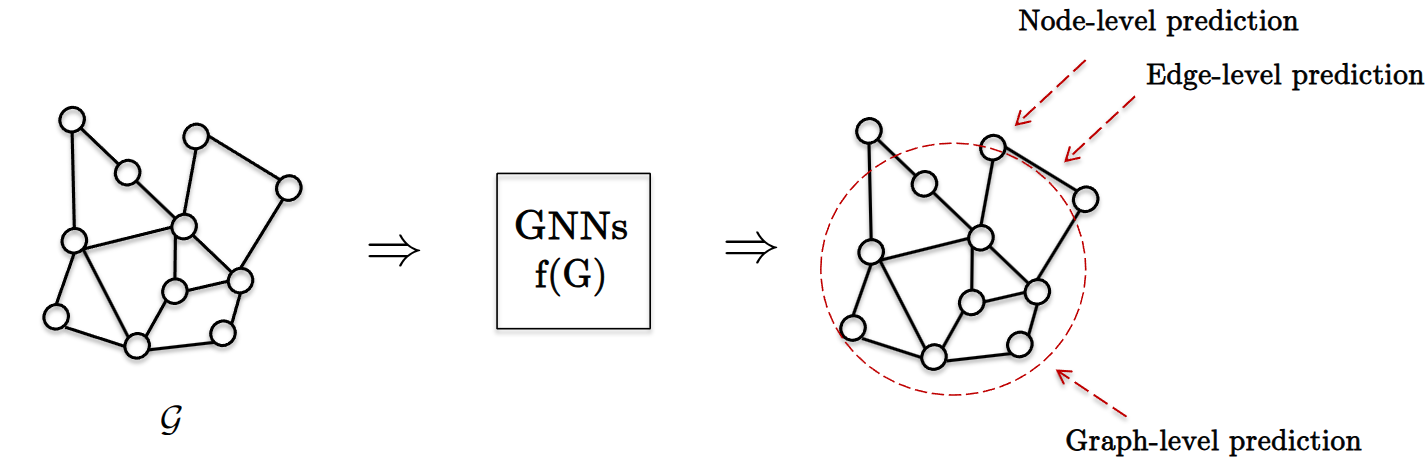
\includegraphics[width=1.0\linewidth]{figures/graph_tasks.png}


\column{0.5\linewidth}

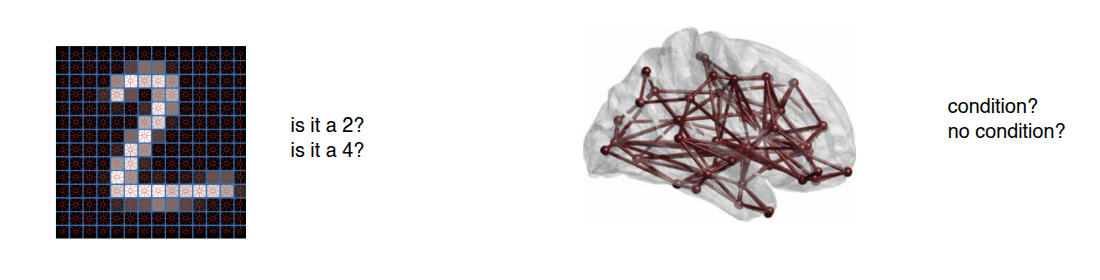
\includegraphics[width=0.9\linewidth]{figures/graph_classification_1.png}

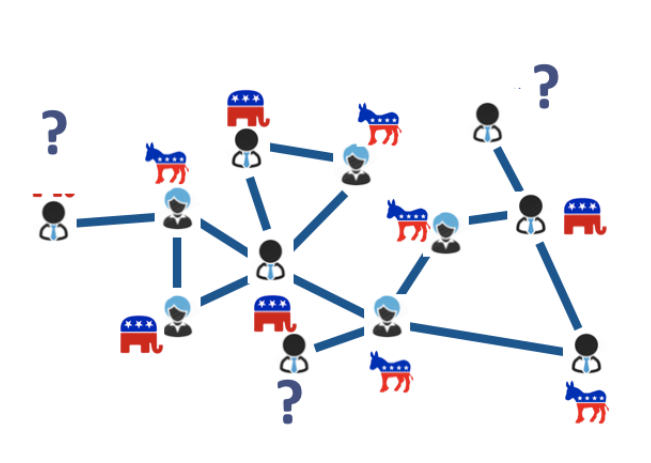
\includegraphics[width=0.5\linewidth]{figures/graph_classification_2.png}

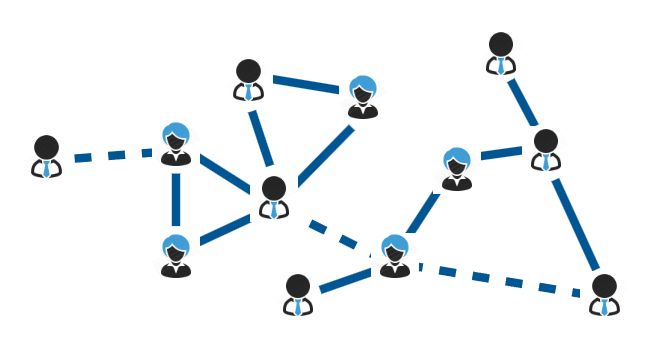
\includegraphics[width=0.5\linewidth]{figures/graph_classification_3.png}

\end{columns}

\end{frame}

\begin{frame}{GNN Case Studies}

\footnotesize


\begin{itemize}
\item Chip design (Google)
\item Resource management
\item Scene reasoning (Meta)
\item Recommendation (UberEats/ Pinterest/ Alibaba)
\item Fake news detection
\item Finance
\item Natural Language Processing
\item Knowledge graphs (Amazon)
\item Transportation (Google Map, Waymo, etc.)
\item Autonomous driving (NVIDIA)
\item Protein \& drug design (Google DeepMind/ Microsoft/ AstraZeneca)
\item Energy physics \& simulations (Google DeepMind)
\item Code bug detection
\item Genomics
\end{itemize}

\end{frame}

\begin{frame}{GNNs for autonomous driving}

\begin{center}
\url{https://slideslive.com/38930570/graph-neural-networks-for-selfdriving}

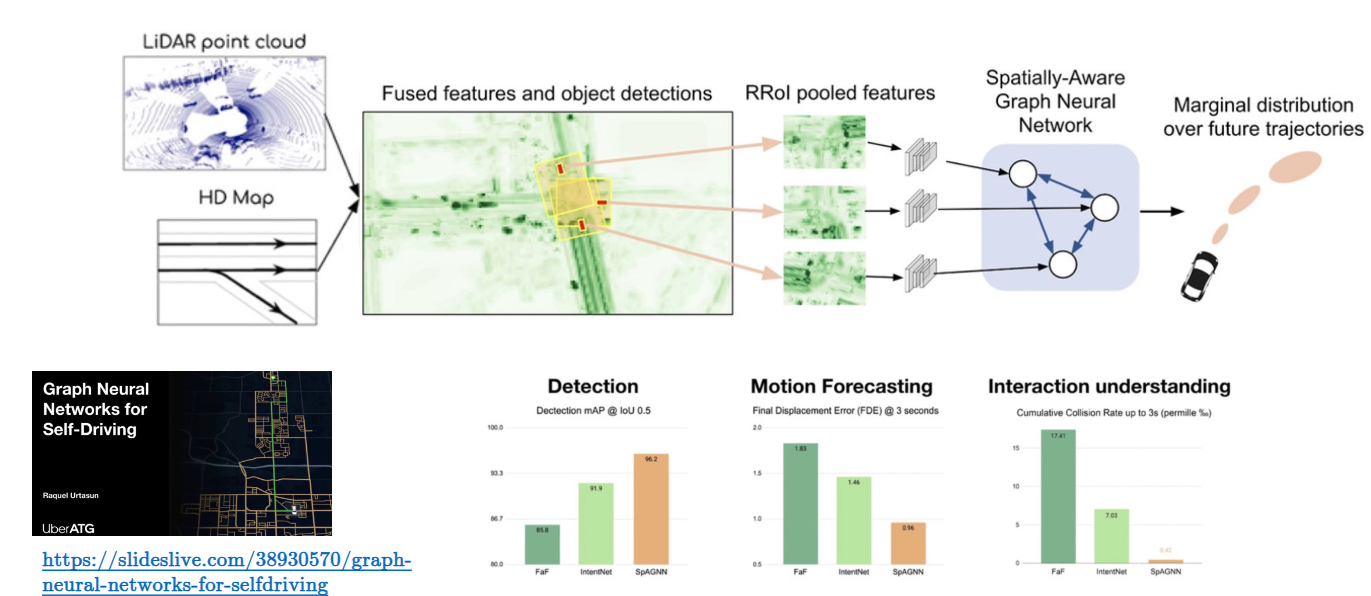
\includegraphics[width=0.85\linewidth]{figures/gnn_av.png}


\end{center}

\end{frame}

\begin{frame}{GNNs for Genomics}

\begin{center}
\url{https://arxiv.org/pdf/2206.00668}

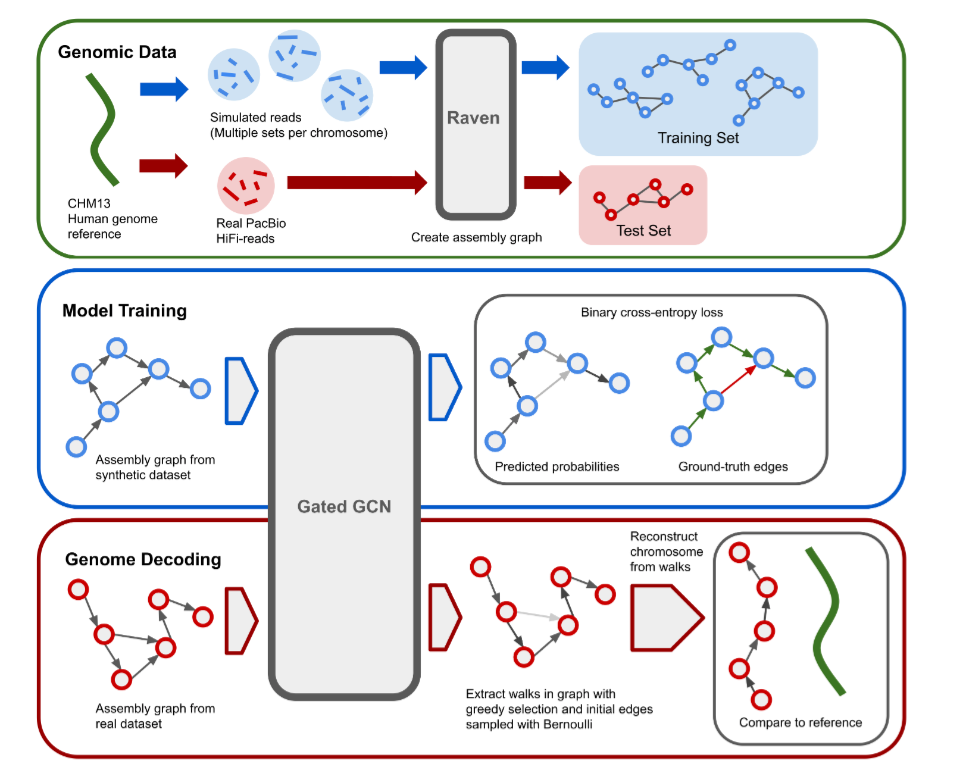
\includegraphics[width=0.5\linewidth]{figures/gnn_genomics.png}


\end{center}

\end{frame}


\begin{frame}{Recommended Textbooks}

\begin{itemize}
\item Graph Representation Learning Book, Springer, 2020 \url{https://github.com/RHxW/CV-DL-Docs/blob/master/GRL_Book.pdf}

\item Geometric Deep Learning: Grids, Groups, Graphs, Geodesics, and Gauges,2021 \url{https://arxiv.org/pdf/2104.13478}

\item Graph Neural Networks: Foundations, Frontiers, Applications, Springer,2022
\url{https://graph-neural-networks.github.io/}

\end{itemize}

\end{frame}

\begin{frame}{GNN Library in PyTorch}

\begin{itemize}
\item PyTorch Geometric
\item Released in March 2019
\item \url{https://pytorch-geometric.readthedocs.io/en/latest/}
\end{itemize}

\end{frame}

\begin{frame}{Graph Categories: Natural Graphs}

Graphs that are not artificially hand-crafted/constructed but just occur by natural process.

\begin{itemize}
\item Social networks : Meta, LinkedIn, Twitter, Tiktok
\item Biological networks : Brain connectivity \& functionality, gene regulatory networks
\item Communication networks : Internet, networking devices
\item Transportation networks : Trains, cars, airplanes, pedestrians
\item Power networks : Electricity, water
\end{itemize}

\begin{center}
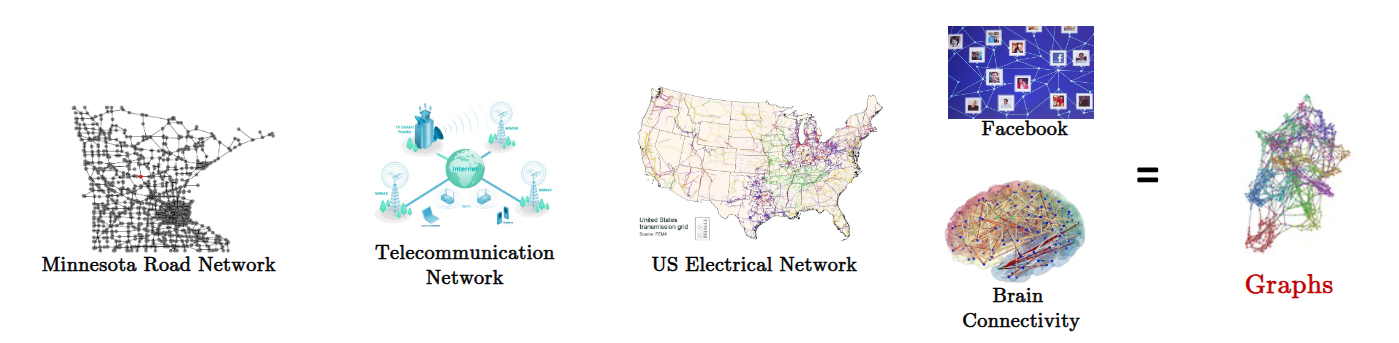
\includegraphics[width=1.0\linewidth]{figures/natural_graphs.png}
\end{center}


\end{frame}

\begin{frame}{Graph Categories: Explicit Graph Construction from Data}

Graphs constructed from data :

\begin{itemize}
\item An example can be: compute the correlation netween samples and treating samples as nodes, form an edge if correlation between two sample is greater than some threshold.
\end{itemize}

\begin{center}
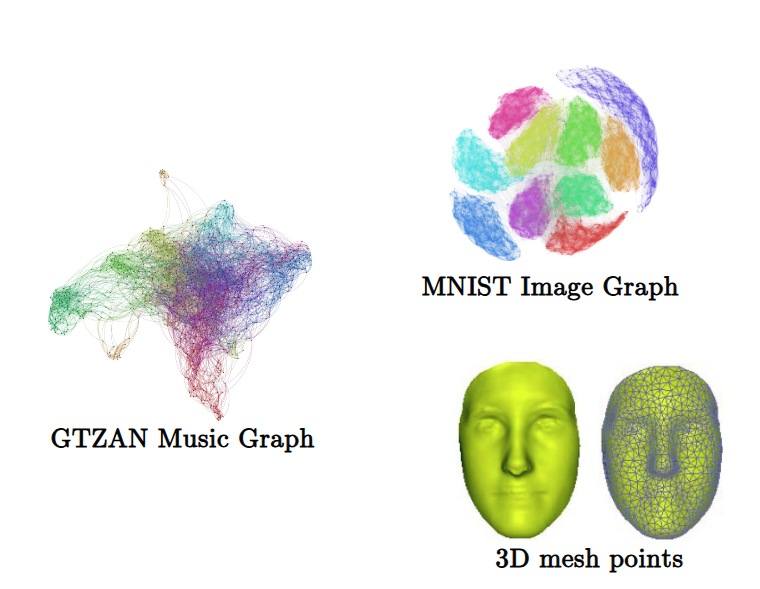
\includegraphics[width=0.45\linewidth]{figures/forced_graph.png}
\end{center}

\end{frame}

\begin{frame}{Adjacency Matrix}

\footnotesize

\begin{columns}

\column{0.5\linewidth}


\begin{itemize}
\item Matrix $A$ in $G = (V,E,A)$ represents structural/topological information about thenetwork. We have two classes of $A$.

\begin{itemize}
\item Binary matrix: $A_{ij} \in \{0,1 \}$


and 

\begin{align*}
A_{ij} = \begin{cases}
1 \quad \quad \text{if} \quad (i, j) \in E\\
 0\quad \quad \text{otherwise} 
 \end{cases}
\end{align*} 

\item Weighted matrix: $A_{ij} \in [0,1]$ : commonly normalized to

\begin{align*}
A_{ij} = \begin{cases}
\in (0, 1] \quad \quad \text{if} \quad (i, j) \in E\\
 0\quad \quad \text{otherwise} 
 \end{cases} 
\end{align*}

\end{itemize}
\end{itemize}

\column{0.5\linewidth}

 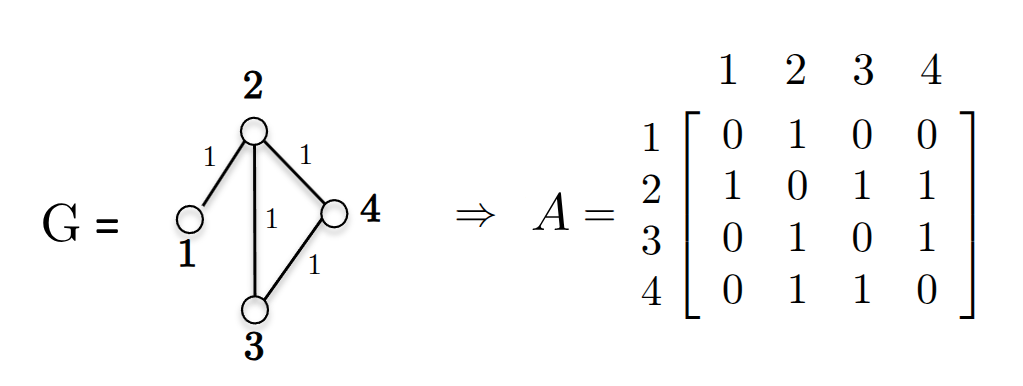
\includegraphics[width=0.95\linewidth]{figures/binary_adjacency.png}
 
 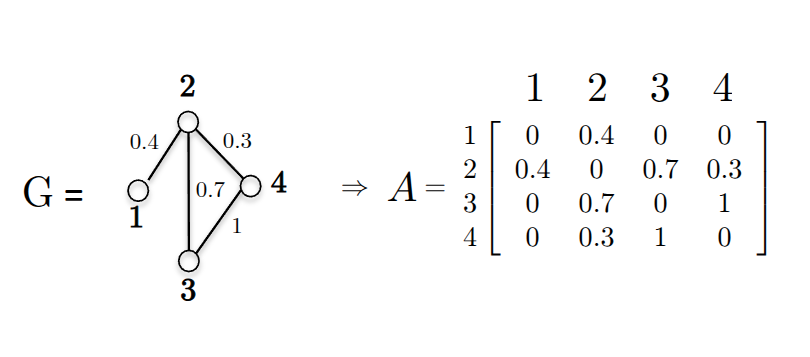
\includegraphics[width=0.95\linewidth]{figures/weighted_adjacency.png}



\end{columns}

\end{frame}



\begin{frame}{Curse of Dimensionality}


\footnotesize

\begin{columns}

\column{0.8\linewidth}


In high dimensions, Euclidean distance between data becomes meaningless.

\vspace{10pt}

If data are uniformly distributed in $\Rbb^d$,then pick any data point $\xbf_i \in V$, that gives

\begin{align*}
\lim_{d\to \infty} \Ebb_{x_i}  \bigg( \frac{d_{max}^{\ell_2}(\xbf_i, V/\ \xbf_i) - d_{min}^{\ell_2}(\xbf_i, V/\ \xbf_i)}{d_{min}^{\ell_2}(\xbf_i, V/\ \xbf_i)}  \bigg)=0
\end{align*}


which just means that all data are really far away to each other with the same distance in a very high-dimensional space.

\begin{itemize}
\item As an example, there is a loss of intuition in high-dimension. 
\item You can think that in Normal distribution, in 1-d, most data are concentrated at the center.
\item But in high-diemsnional spaces, most data are concentrated on the surface.
\end{itemize}

\end{columns}

\end{frame}

\begin{frame}{But Then There Might Be Some Structure in High-Dimension}

\begin{itemize}
\item \textbf{Data are uniformly distributed} is actually not true for real-world data.
\item Data have always properties, i.e. structures or invariances, such that they belong to a low-dimensional space called manifold where (geodesic) distances are meaningful.
\end{itemize}

 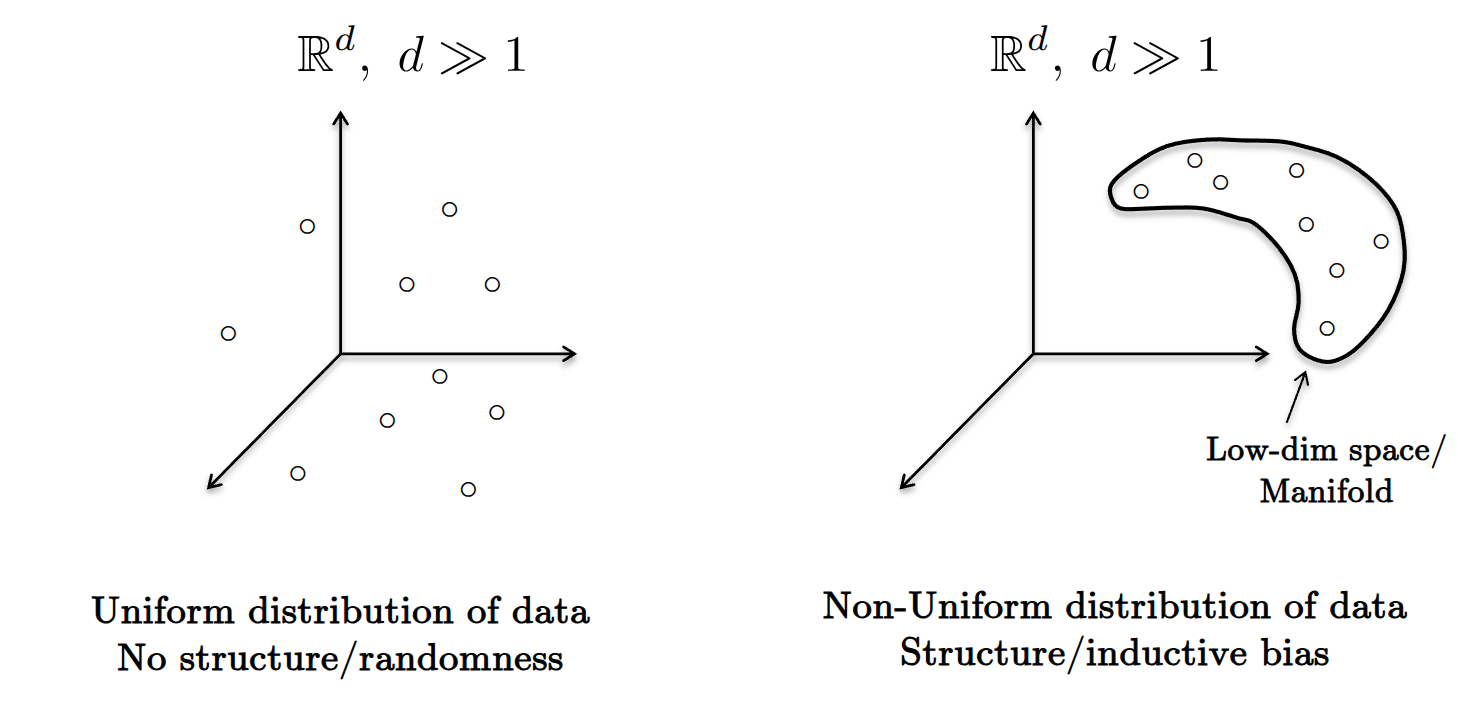
\includegraphics[width=0.95\linewidth]{figures/manifold_distribution.png}


\end{frame}

\begin{frame}{Manifold Learning}

\begin{center}
A class of algorithms that extracts low-dimensional patterns is manifold learning.
\end{center}


 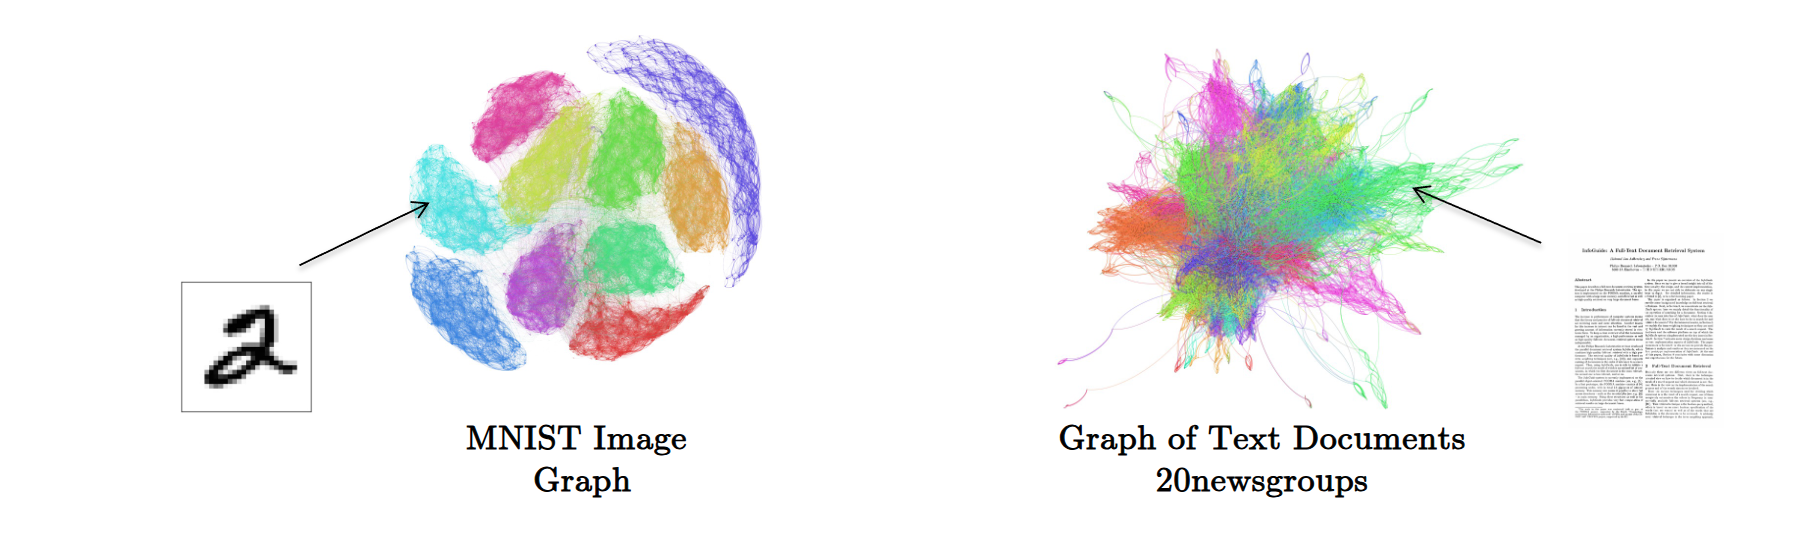
\includegraphics[width=0.95\linewidth]{figures/manifold_learning.png}


\end{frame}


\begin{frame}{Manifolds to Graphs}


\begin{columns}

\column{0.65\linewidth}


\begin{center}
\textbf{Primary assumption:} High-dimensional data are sampled froma low-dimensional manifold.

\vspace{10pt}

\textbf{Example:}   Let $x$ be a movie, each movie is defined by $d$ features/attributes like genre, actors, release year, origin country, etc such that $\xbf$ in $\Rbb^d$. We can decide to make theassumption that all movies form a manifold $\Mcal$ in $\Rbb^d$.
\end{center}

\column{0.35\linewidth}

 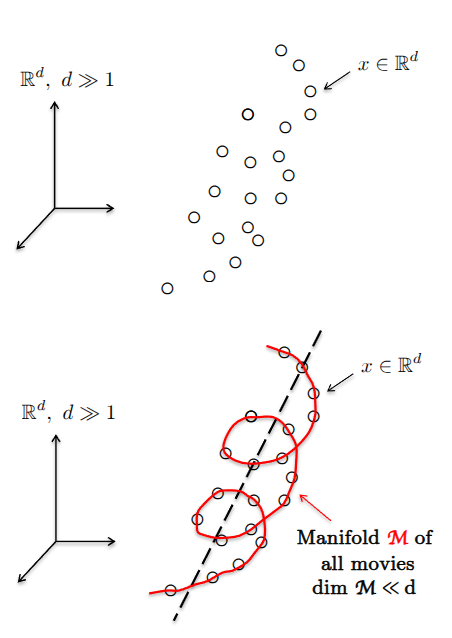
\includegraphics[width=0.95\linewidth]{figures/manifold_to_graph.png}
\end{columns}

\end{frame}


\begin{frame}{From Manifolds to Graphs}

Graphs can be regarded as a manifold sampling process.

\begin{itemize}
\item The manifold information is represented by a neighborhood graph (observe that themanifold is never directly observed or constructed).
\end{itemize}

 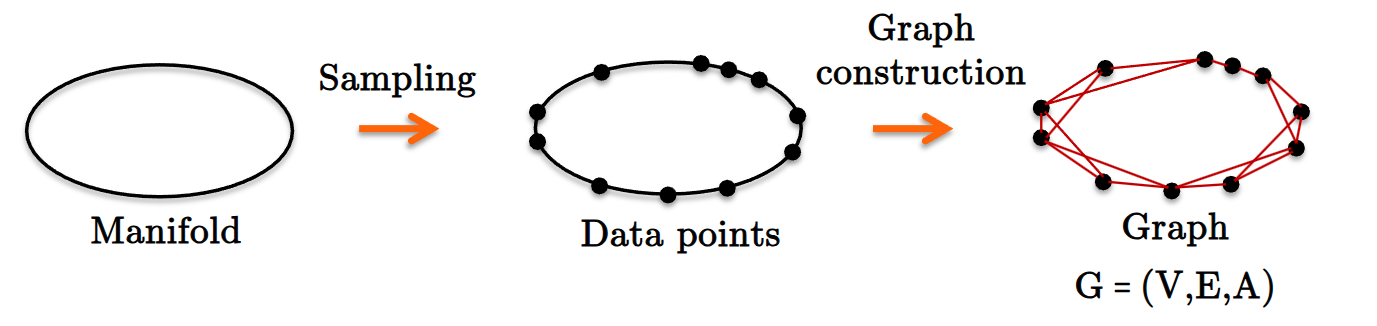
\includegraphics[width=0.95\linewidth]{figures/manifold_construction.png}

\end{frame}

\begin{frame}{Neighborhood Graphs}

\begin{itemize}
\item Most populars are $k-NN$ graphs defined as :

\begin{align*}
A_{ij} = \begin{cases}
e^{-\frac{dis(\xbf_i, \xbf_j)^2}{\sigma^2}} \quad \text{~~~if~~~} j \in \Ncal_i^k\\
0 \quad \text{~~~otherwise~~~}
\end{cases}
\end{align*}
where $dist(\xbf_t, \xbf_j)$ cane be any kind of distance. $\Ncal_i^k$ is the neighborhood of data $\xbf_i$.
\end{itemize}

 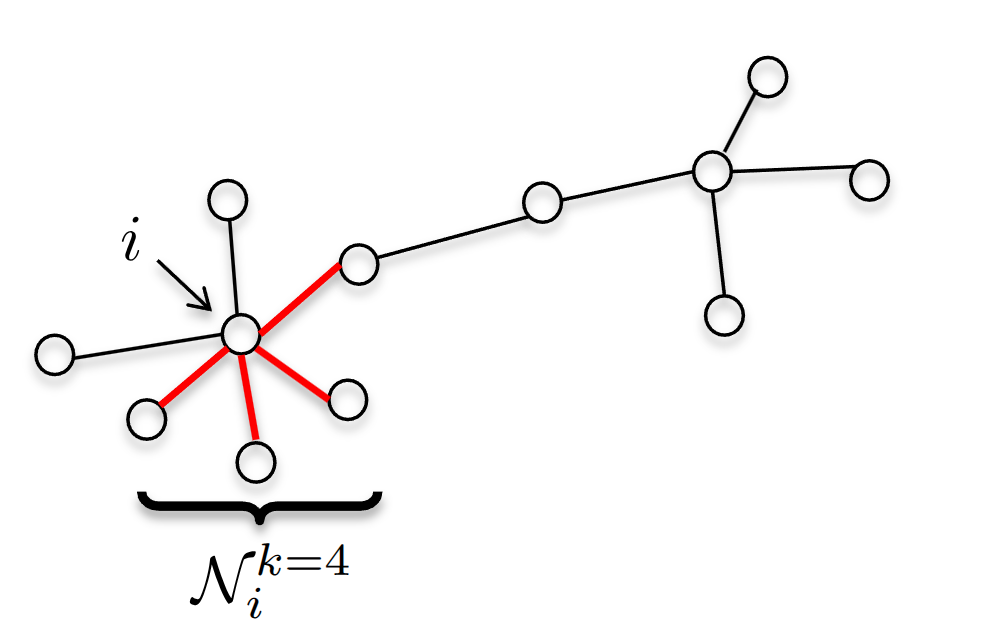
\includegraphics[width=0.45\linewidth]{figures/knn_graph.png}


\end{frame}

\begin{frame}{Spectral Graph Theory}

\footnotesize

Spectral graph theory (SGT) can

\begin{itemize}
\item find meaningful patterns that reveal multi-scale graph structures.
\item Process data defined on the graph domain (a.k.a. graph signal processing).
\item Boost performance of learning tasks s.a. clustering, classification, recommendation, etc.
\end{itemize}


\vspace{10pt}

\textbf{Graph Laplacian Operator $L$.}
\begin{itemize}
\item Central operator of diffusion processes on graphs.
\item Basis functions of this operator are the well-known Fourier modes
\end{itemize}

 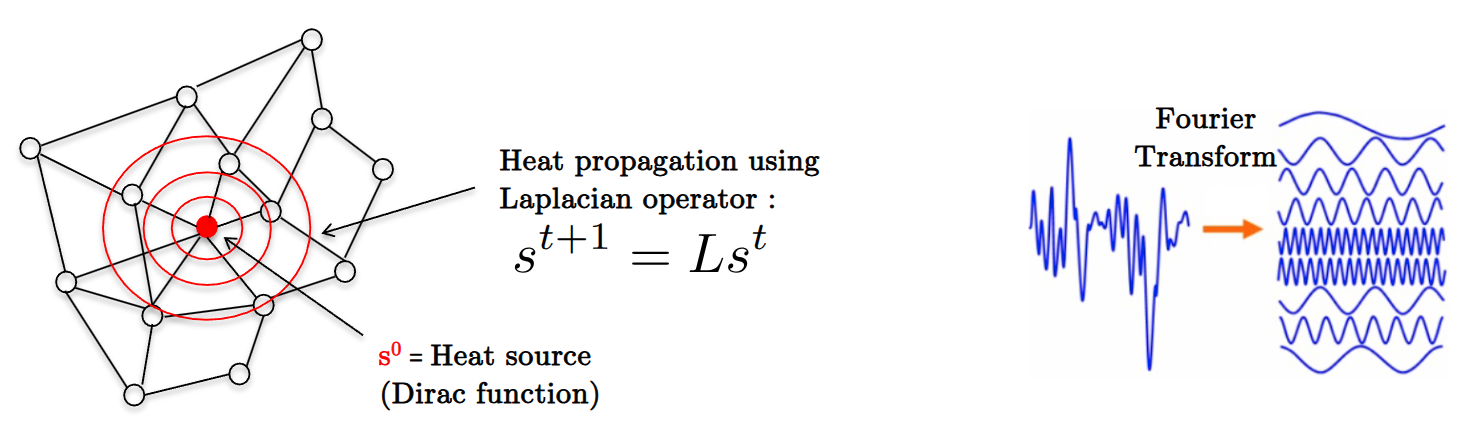
\includegraphics[width=0.55\linewidth]{figures/Laplacian_Fourier.png}


\end{frame}

\begin{frame}{Graph Laplacian}

\begin{itemize}
\item Unnormalized Graph Laplacian:

\begin{align*}
L = D - A
\end{align*}

where $D$ is the degree matrix : $D = diag(d_1, \cdots, d_n)$, and $d_ii = \sum_j A_{ij}$.

\item Normalized Laplacian

\begin{align*}
L_n = D^{-1/2} L D^{-1/2} = I_n - D^{-1/2}A D^{-1/2}
\end{align*}

\item Random Walk Laplacian:

\begin{align*}
L_w = D^{-1}L = I_n - D^{-1}A
\end{align*}

\item All Laplacians are diffusion operators.
\end{itemize}

\end{frame}


\begin{frame}{}


\begin{center}
\url{https://docs.google.com/presentation/d/1psyAe3x8A67eM0eauX34Ii9igefC1124/edit?usp=sharing&ouid=102329043416263329658&rtpof=true&sd=true}

\end{center}
\end{frame}

\end{document}